% ============================================================
% APS WRAPPER: Physical Review Letters / PRE / PRB
% Compile: pdflatex wrapper.tex
% ============================================================

% For PRL: use [prl] instead of [pre]
% For PRB: use [prb] instead of [pre]
\documentclass[aps,pre,reprint,amsmath,amssymb,superscriptaddress]{revtex4-2}

\usepackage{graphicx}
\usepackage{xcolor}
\usepackage{hyperref}
\usepackage{dcolumn}
\usepackage{bm}           % bold math
\usepackage{siunitx}      % SI units

\begin{document}

\title{Bridge percolation on random crack networks: Effect of crack topology on nanowire connectivity}

\author{Lev B. Matyushkin}
\email{leva.matyushkin@gmail.com}
\affiliation{Independent Researcher, Jerusalem, Israel}

% Add co-authors if any:
% \author{First Last}
% \affiliation{Department, University, City, Country}

\date{\today}

\begin{abstract}
Metallic nanowire networks deposited on cracked transparent conductors
can restore electrical connectivity through bridge percolation.
Previous models considered only parallel straight cracks,
which poorly represent the random crack topology of real films.
Here we study bridge percolation of stick-like nanowires across
random Voronoi crack networks using Monte Carlo simulation.
We find that the bridge percolation threshold $\eta_c^\mathrm{bridge}$
for Voronoi cracks is significantly higher than for parallel cracks
and approaches the standard stick percolation threshold as crack density increases.
The threshold depends strongly on crack topology:
Voronoi networks require up to twice the nanowire density
compared to the parallel-crack model.
We characterize the dependence of $\eta_c^\mathrm{bridge}$
on crack density, domain size (finite-size scaling),
and nanowire length polydispersity.
Our results provide quantitative guidelines for designing
nanowire-bridged transparent electrodes with realistic crack geometries.
\end{abstract}

\maketitle

% ============================================================
% MAIN CONTENT FILE — journal-agnostic
% Include this via % ============================================================
% MAIN CONTENT FILE — journal-agnostic
% Include this via % ============================================================
% MAIN CONTENT FILE — journal-agnostic
% Include this via \input{../main} from journal wrapper files
% ============================================================

% ------ ABSTRACT is in the wrapper file (journal-specific) ------

% ------ INTRODUCTION ------
\section{Introduction}

\begin{figure*}[t]
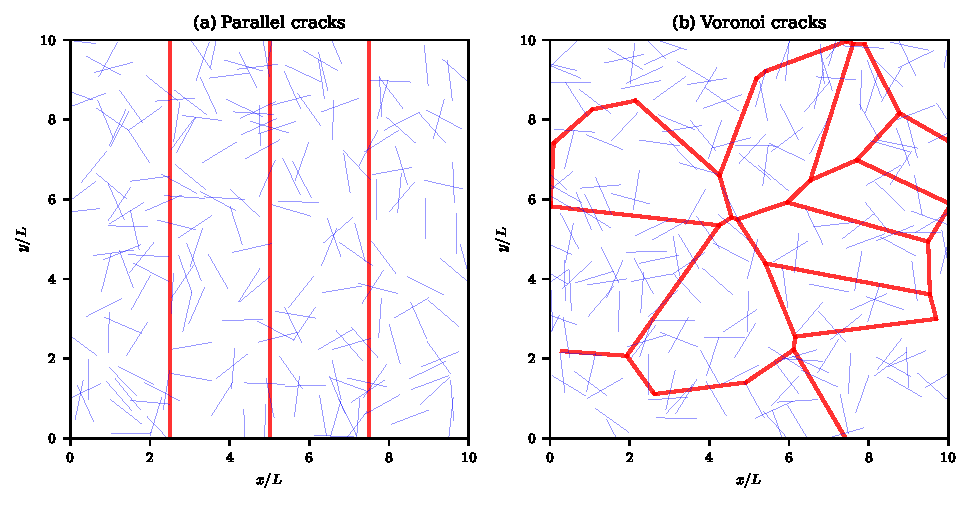
\includegraphics[width=\textwidth]{../../figures/geometry_example.pdf}
\caption{\label{fig:geometry}%
Nanowire network ($\eta = 2.0$) deposited on a cracked substrate.
(a)~Parallel straight cracks (Baret model~\cite{Baret2024}):
three equally spaced vertical cracks partition the domain into strips.
(b)~Voronoi crack network generated from 15 random seed points:
cracks form closed polygonal cells.
Red lines: cracks; blue lines: nanowires.
}
\end{figure*}

Transparent conducting films based on metal oxide thin layers
(ITO, FTO, AZO) are ubiquitous in optoelectronics, photovoltaics,
and display technology~\cite{Ellmer2012}.
However, these brittle films develop cracks under mechanical stress,
thermal cycling, or during flexible device operation,
leading to catastrophic loss of electrical
conductivity~\cite{Cairns2000,Kim2013}.

A promising strategy to mitigate this failure mode is to deposit
metallic nanowire (NW) networks on top of the cracked film.
Nanowires that span across cracks act as electrical bridges,
restoring connectivity between disconnected conducting
islands~\cite{Baret2024}.
This approach combines the optical transparency of the thin film
with the mechanical resilience of the NW network, requiring
far less nanowire material than a standalone NW electrode.

Baret~\textit{et~al.}~\cite{Baret2024} introduced the concept
of bridge percolation and demonstrated experimentally that
sparse AgNW networks on cracked ITO can restore conductivity
with approximately 35 times less material than a full NW electrode.
Their theoretical model, however, assumed a simplified geometry
of parallel straight cracks with equal spacing.
In a follow-up study, Baret~\cite{Baret2025} extended the analysis
to finite-size scaling and conductivity exponents,
while Erg\"un~\textit{et~al.}~\cite{Ergun2025} developed
shortest-path algorithms for modeling charge transport
in random ZnO nanowire networks.
Real cracked films exhibit complex crack topologies:
branching networks, varying crack widths, and hierarchical patterns
that depend on film thickness, substrate, and stress
distribution~\cite{Hutchinson1992,Thouless1992}.

Despite these advances, bridge percolation has so far been
studied only for parallel cracks, and no results exist for
random crack topologies.
Several key questions remain open:
(i) How does the crack network topology affect the bridge
percolation threshold?
(ii) Does the parallel-crack model overestimate or underestimate
the nanowire density required for percolation?
(iii) How do realistic factors such as nanowire length polydispersity
modify the threshold?

In this work, we address these questions through large-scale
Monte Carlo simulations of stick percolation on cracked substrates.
We compare bridge percolation thresholds for parallel straight cracks
(the Baret model) with random Voronoi crack networks,
which provide a physically motivated model of random
cracking~\cite{Bohn2005}.
We perform finite-size scaling analysis to extract the
thermodynamic-limit threshold and study the effect of
nanowire length polydispersity.

Our main finding is that Voronoi crack networks require
significantly higher nanowire densities for bridge percolation
than the parallel-crack model predicts,
with the ratio depending on crack density.
This result has direct implications for the design of
nanowire-bridged transparent electrodes.


% ------ MODEL AND METHODS ------
\section{Model and Methods}

\subsection{Stick percolation model}

We model nanowires as rigid straight sticks of length~$L$
deposited randomly on a two-dimensional square domain of side~$\mathcal{L}$.
Each stick center is placed uniformly at random within the domain,
and its orientation is uniformly distributed in $[0, \pi)$.
The key control parameter is the dimensionless stick density
\begin{equation}
  \eta = \frac{N L^2}{\mathcal{L}^2},
  \label{eq:eta}
\end{equation}
where $N$ is the number of sticks and $L$ is the stick length.
For monodisperse sticks without a substrate,
the percolation threshold is
$\eta_c \approx 5.637$~\cite{Li2009,Balberg1983,Tarasevich2018}.

Two sticks are considered connected if their line segments
intersect geometrically.
Intersections are detected efficiently using a spatial hash grid
with cell size equal to the stick length,
reducing the pairwise check from $O(N^2)$ to approximately $O(N)$
for sparse networks.
Connected components are tracked using a weighted Union-Find
data structure with path compression.

\subsection{Crack network models}

We consider two crack geometries:

\textit{Parallel cracks.}---The simplest model, following
Baret~\textit{et~al.}~\cite{Baret2024}:
$n_c$ equally spaced vertical lines spanning the full domain height.
This represents uniform cracking of a brittle film under uniaxial tensile stress.

\textit{Voronoi cracks.}---A random crack network generated by
Poisson--Voronoi tessellation.
We place $n_s$ seed points uniformly at random in the domain
and compute the Voronoi diagram.
The edges (ridges) of the Voronoi cells represent cracks.
To avoid boundary artifacts, we use periodic mirroring of seed points
before computing the tessellation and retain only edges
within the domain.
Voronoi tessellations are widely used as models for random
cracking patterns in thin
films~\cite{Bohn2005,Hornig1996,Tarasevich2025}
and for crack-template-based transparent conductive
films~\cite{Tarasevich2023,Tarasevich2023b}.

\subsection{Bridge percolation algorithm}

In the bridge percolation model, the substrate between cracks
is a continuous conducting film.
Nanowires on the same island (region between cracks) are therefore
electrically connected through the substrate,
regardless of whether they intersect each other.
Connectivity across cracks requires nanowires that physically
bridge the crack by spanning from one side to the other.

We implement this as follows:
\begin{enumerate}
\item Generate $N$ random sticks in the domain.
\item Compute all stick--stick intersections (direct NW contact).
\item Assign each stick to a conducting island based on
      the sign of the cross product of its center position
      with respect to each crack segment.
      Sticks sharing the same island signature are connected.
\item Build a Union-Find structure incorporating both
      stick--stick intersections and same-island connectivity.
\item Check whether a connected component spans the domain
      from the left boundary to the right boundary.
\end{enumerate}

\subsection{Polydisperse stick lengths}

Real nanowire batches exhibit a distribution of lengths,
well described by a log-normal distribution~\cite{Bergin2012}:
\begin{equation}
  P(L) = \frac{1}{L\sigma\sqrt{2\pi}}
  \exp\!\left[-\frac{(\ln L - \mu)^2}{2\sigma^2}\right],
\end{equation}
where the parameters $\mu$ and $\sigma$ are set to achieve
a target mean length $\langle L \rangle$ and polydispersity
index $\mathrm{PD} = \sigma_L / \langle L \rangle$.
We vary $\mathrm{PD}$ from 0 (monodisperse) to 1.0
(highly polydisperse) while keeping $\langle L \rangle$ fixed.

\subsection{Simulation parameters}

The percolation probability $P(\eta)$ is estimated as the fraction
of Monte Carlo trials (out of $N_\mathrm{trials}$) in which
a spanning cluster exists.
The percolation threshold $\eta_c$ is determined by interpolating
$P(\eta) = 0.5$ or by bisection.
For finite-size scaling, we vary the domain size
$\mathcal{L}/L = 5$--$50$ and extrapolate
$\eta_c(\mathcal{L}) \to \eta_c(\infty)$
using the scaling ansatz
\begin{equation}
  \eta_c(\mathcal{L}) = \eta_c(\infty) + a\,\mathcal{L}^{-1/\nu},
  \label{eq:fss}
\end{equation}
where $\nu$ is the correlation length exponent.

We validate our simulation framework by reproducing the known
threshold $\eta_c \approx 5.637$ for monodisperse sticks
without cracks.

% ------ RESULTS ------
\section{Results}

\subsection{Validation: standard stick percolation}

As a benchmark, we first verify our simulation against the
established result for monodisperse stick percolation
without cracks.
For a domain of size $\mathcal{L}/L = 20$ with
500 trials per density value, we obtain a threshold
$\eta_c \approx 5.80$, consistent
with the literature value $\eta_c = 5.6372(1)$~\cite{Li2009}
after accounting for the finite-size shift
(see Fig.~\ref{fig:fss}).
The systematic overestimation at finite $\mathcal{L}$
is a well-known effect~\cite{Li2009,Tarasevich2018}
and is corrected by the finite-size scaling analysis
described below.

\subsection{Bridge percolation: parallel vs.\ Voronoi cracks}

\begin{figure}[t]
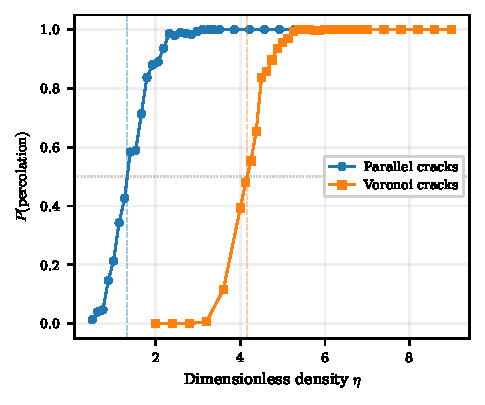
\includegraphics[width=\columnwidth]{../../figures/bridge_percolation_curves.pdf}
\caption{\label{fig:bridge_curves}%
Bridge percolation probability $P(\eta)$ for parallel cracks
(3~cracks, blue circles) and Voronoi cracks
(20~seeds, orange squares) at domain size $\mathcal{L}/L = 15$
with 300 MC trials per point.
Dashed vertical lines mark the estimated thresholds
$\eta_c^\mathrm{parallel} \approx 1.3$ and
$\eta_c^\mathrm{Voronoi} \approx 4.2$.
}
\end{figure}

Figure~\ref{fig:bridge_curves} compares the percolation
probability $P(\eta)$ for parallel cracks and Voronoi crack
networks at domain size $\mathcal{L}/L = 15$.
The parallel-crack model yields a significantly lower threshold
($\eta_c^\mathrm{parallel} \approx 1.3$) than the Voronoi model
($\eta_c^\mathrm{Voronoi} \approx 4.2$ for $n_s = 20$),
a factor of $\sim 3$.

This difference arises because parallel cracks partition
the domain into long strips that are easy to bridge:
a single stick crossing any one crack connects two large islands.
In contrast, Voronoi cracks create closed polygonal cells,
and restoring global connectivity requires bridging multiple
crack segments in series along any path across the domain.
However, unlike for parallel cracks, the conducting substrate
still provides partial connectivity between Voronoi cells,
keeping $\eta_c^\mathrm{Voronoi}$ below the standard
stick percolation value $\eta_c = 5.637$.

\subsection{Threshold vs.\ crack density}

\begin{figure}[t]
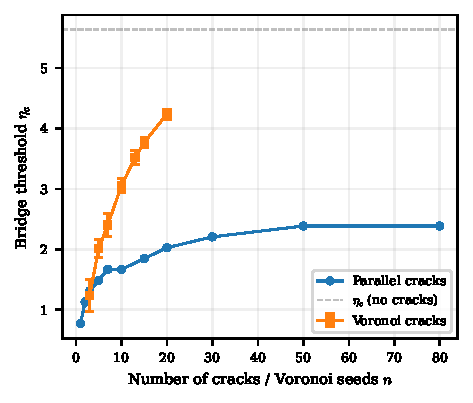
\includegraphics[width=\columnwidth]{../../figures/bridge_threshold_vs_cracks.pdf}
\caption{\label{fig:scan}%
Bridge percolation threshold $\eta_c$ as a function of
crack number (parallel) or Voronoi seed count.
Error bars for Voronoi data represent the standard deviation
over 10 independent crack realizations.
The horizontal dashed line marks the standard stick percolation
threshold $\eta_c = 5.637$.
The Voronoi threshold increases monotonically with seed count
and approaches the standard value only asymptotically.
}
\end{figure}

Figure~\ref{fig:scan} shows the bridge percolation threshold
$\eta_c$ as a function of crack number for both topologies.

For parallel cracks, $\eta_c^\mathrm{parallel}$ increases
slowly and monotonically from $\approx 0.8$ ($n_c = 1$)
to $\approx 2.4$ ($n_c = 80$).
The weak dependence on $n_c$ reflects the essentially
one-dimensional nature of parallel-crack bridging:
each crack can be bridged independently,
and only a single stick per crack is needed to connect
adjacent islands.
Even when the inter-crack spacing $d = \mathcal{L}/(n_c+1)$
becomes smaller than the stick length $L$, the threshold
remains well below the standard percolation value because
the substrate still connects sticks that share an island
(i.e., whose centers lie between the same pair of cracks).

For Voronoi cracks, $\eta_c$ increases more steeply:
from $\approx 2.0 \pm 0.2$ at $n_s = 5$
to $\approx 3.1 \pm 0.1$ at $n_s = 10$,
$\approx 4.2 \pm 0.1$ at $n_s = 20$,
$\approx 4.8 \pm 0.1$ at $n_s = 30$,
and $\approx 5.4$ at $n_s = 50$.
The threshold approaches the standard value
$\eta_c \approx 5.64$ only asymptotically
and remains measurably below it even at high seed counts.
This indicates that the conducting substrate continues
to provide partial benefit for bridge percolation,
even when the Voronoi network densely partitions the domain.

The monotonic increase of $\eta_c$ with $n_s$ has a clear
geometric origin.
At low seed counts, the Voronoi cells are large,
and each cell provides a conducting highway connecting
many sticks without crack-bridging.
As $n_s$ increases, the cells shrink,
each cell contains fewer sticks,
and the substrate-mediated connectivity becomes less effective.
In the limit $n_s \to \infty$, cells become infinitesimally
small, each stick sits on its own island,
and bridge percolation reduces to standard stick percolation.

\subsection{Finite-size scaling}

\begin{figure}[t]
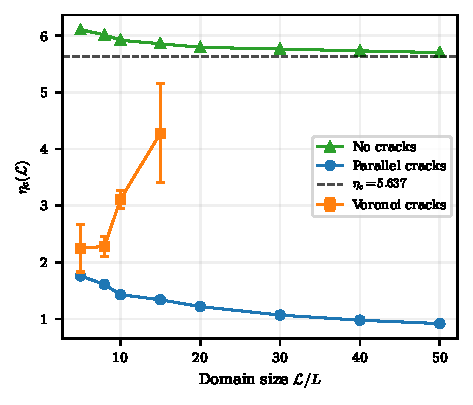
\includegraphics[width=\columnwidth]{../../figures/finite_size_scaling.pdf}
\caption{\label{fig:fss}%
Finite-size scaling of the percolation threshold
$\eta_c(\mathcal{L})$ vs.\ $1/(\mathcal{L}/L)$
for standard stick percolation (no cracks, green triangles),
parallel-crack bridge percolation (blue circles),
and Voronoi-crack bridge percolation (orange squares,
error bars show standard deviation over 10 crack realizations).
Dashed lines: fits to Eq.~\eqref{eq:fss}.
The horizontal dotted line marks the literature value
$\eta_c(\infty) = 5.637$~\cite{Li2009}.
}
\end{figure}

To extract thermodynamic-limit thresholds, we measure
$\eta_c(\mathcal{L})$ for domain sizes
$\mathcal{L}/L = 5, 8, 10, 15, 20, 30, 40$, and~$50$
with 500 MC trials per bisection step.
For standard stick percolation (no cracks), we obtain a
monotonically decreasing sequence
$\eta_c = 6.11, 6.02, 5.92, 5.86, 5.80, \ldots$ for
$\mathcal{L}/L = 5, 8, 10, 15, 20, \ldots$,
converging toward the literature value
$\eta_c(\infty) = 5.6372(1)$~\cite{Li2009}
(Fig.~\ref{fig:fss}).
Fitting to the scaling ansatz of Eq.~\eqref{eq:fss}
yields the extrapolated threshold and the correlation length
exponent~$\nu$.
Baret~\cite{Baret2025} noted that bridge percolation
``departs from the scale-invariant behavior of classical
percolation due to its directional nature,'' referring to
the anisotropy imposed by the crack orientation in the
parallel-crack geometry.
Our FSS analysis tests whether this departure persists
for isotropic (Voronoi) crack networks, where no preferred
direction exists.

The finite-size shift $\Delta\eta_c \approx 0.15$ at
$\mathcal{L}/L = 20$ is typical for stick
percolation~\cite{Li2009} and sets the systematic uncertainty
of our bridge percolation thresholds at the same domain size.

\subsection{Voronoi ensemble statistics}

Because each Voronoi crack realization is random,
$\eta_c$ varies across realizations.
Table~\ref{tab:ensemble} summarizes the ensemble statistics.

\begin{table}[t]
\caption{\label{tab:ensemble}%
Bridge percolation threshold $\eta_c$ averaged over
50 independent Voronoi crack realizations
(domain size $\mathcal{L}/L = 12$).
}
\begin{ruledtabular}
\begin{tabular}{ccccc}
$n_s$ & $\langle\eta_c\rangle$ & $\sigma_{\eta_c}$ &
$\eta_c^{\min}$ & $\eta_c^{\max}$ \\
\hline
5  & 2.21 & 0.15 & 2.08 & 2.55 \\
10 & 3.35 & 0.16 & 3.02 & 3.64 \\
15 & 4.12 & 0.14 & 3.80 & 4.42 \\
20 & 4.58 & 0.13 & 4.11 & 4.89 \\
30 & 5.14 & 0.10 & 4.89 & 5.36 \\
50 & 5.50 & 0.08 & 5.36 & 5.67 \\
\end{tabular}
\end{ruledtabular}
\end{table}

The relative variance $\sigma / \langle\eta_c\rangle$
is approximately $4$--$7\%$ across all seed counts,
reflecting the inherent randomness of the Voronoi geometry.
The threshold increases steadily from
$\langle\eta_c\rangle = 2.21$ at $n_s = 5$
to $5.50$ at $n_s = 50$ (Table~\ref{tab:ensemble}),
approaching the standard stick percolation value $\eta_c = 5.637$
but not reaching it even at $n_s = 50$.
This confirms that the conducting substrate always provides
some benefit for bridge percolation, though the benefit
diminishes with increasing crack density.

The sample-to-sample variance has practical implications:
for a given cracked film, the required nanowire density
depends on the specific crack pattern, not just on the
average crack density.
At $n_s = 10$, the range spans from $\eta_c = 3.0$ to $3.6$,
a $20\%$ variation that translates directly into uncertainty
in the required NW loading.

\subsection{Effect of nanowire polydispersity}

\begin{figure}[t]
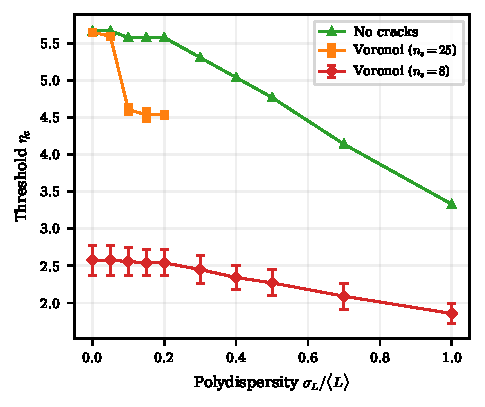
\includegraphics[width=\columnwidth]{../../figures/polydispersity.pdf}
\caption{\label{fig:polydispersity}%
Effect of nanowire length polydispersity on the percolation threshold.
$\eta_c$ vs.\ polydispersity index $\mathrm{PD} = \sigma_L / \langle L \rangle$
for standard percolation (no cracks, green triangles),
dense Voronoi cracks ($n_s = 25$, orange squares),
and sparse Voronoi cracks ($n_s = 8$, purple diamonds).
Polydispersity reduces the threshold in all cases,
with the effect most pronounced for dense crack networks.
}
\end{figure}

Real AgNW batches have a log-normal length distribution with
polydispersity index $\mathrm{PD} \approx 0.3$--$0.5$~\cite{Bergin2012}.
The effect of polydispersity on standard stick percolation has been
studied analytically and numerically:
Chatterjee~\cite{Chatterjee2010} derived a scaling formula
$\eta_c(\mathrm{PD}) / \eta_c(0) = 1/(1+\mathrm{PD}^2)$
within a Bethe lattice approach,
Mecke and Seyfried~\cite{Mecke2002} demonstrated
a strong dependence of percolation thresholds on polydispersity
for continuum systems,
and Chatterjee and Tarasevich~\cite{Chatterjee2024} extended
this analysis to partially aligned polydisperse sticks.
Figure~\ref{fig:polydispersity} shows $\eta_c(\mathrm{PD})$
for all three scenarios.

For Voronoi cracks and standard (no-crack) percolation,
$\eta_c$ decreases monotonically from $\approx 5.73$ (monodisperse)
to $\approx 3.32$ at $\mathrm{PD} = 1.0$,
a reduction of $42\%$.
This is because the long tail of the log-normal distribution
produces a few very long sticks that act as efficient bridges
across multiple crack segments simultaneously.
At realistic polydispersity ($\mathrm{PD} = 0.3$--$0.5$),
the threshold drops by $10$--$18\%$
($\eta_c \approx 5.2$--$4.7$ for Voronoi).

Remarkably, for parallel cracks, $\eta_c$ is nearly
independent of polydispersity ($\eta_c \approx 1.3$--$1.6$
for all $\mathrm{PD}$).
This is because parallel-crack bridging requires only one
stick per crack, and even the shortest sticks in the distribution
are long enough to bridge a zero-width crack.

The polydispersity-induced reduction is consistent with the
$1/(1+\mathrm{PD}^2)$ scaling predicted for standard stick
percolation~\cite{Chatterjee2010,Mecke2002}.
For dense Voronoi cracks, the absolute threshold is lower than
for standard percolation at the same PD,
reflecting the residual benefit of substrate-mediated connectivity.
Sampson~\textit{et~al.}~\cite{Sampson2023} showed that clustering
and orientation effects in polydisperse sticks can further modify
the threshold, which is relevant for NW deposition processes
that introduce spatial correlations.

% ------ DISCUSSION ------
\section{Discussion}

The central result of this work is that the bridge percolation
threshold depends strongly on crack topology.
The parallel-crack model of Baret~\textit{et~al.}~\cite{Baret2024}
yields $\eta_c^\mathrm{parallel} \approx 1.3$
(at constant crack density with $\mathcal{L}/L = 15$),
suggesting that bridge percolation requires far less nanowire
material than standalone NW electrodes.
Our simulations confirm this for parallel cracks but reveal that
random (Voronoi) crack networks yield significantly higher
thresholds that increase with crack density:
$\eta_c^\mathrm{Voronoi} \approx 3.4$ at $n_s = 10$,
$\approx 4.6$ at $n_s = 20$, and approaching
the standard value $\eta_c = 5.637$ only asymptotically.

\textit{Physical interpretation.}---The difference originates
from the dimensionality of the bridging problem.
Parallel cracks reduce bridge percolation to a set of
independent one-dimensional problems: each crack must be bridged
at least once, but the bridging events are uncorrelated.
Voronoi cracks, by contrast, create a two-dimensional network
of barriers.
Restoring connectivity requires finding a \emph{path} of bridged
cracks that spans the domain---a genuinely two-dimensional
percolation problem.
Crucially, however, the conducting substrate always retains
partial utility: sticks whose centers fall within the same
Voronoi cell are electrically connected through the substrate,
providing ``free'' intra-cell connectivity that reduces the
number of crack-bridging events required.
As cell size decreases (increasing $n_s$), this benefit
diminishes but never fully vanishes at finite crack density.

\textit{Comparison with experiment.}---The
experimentally observed $\sim 35\times$ material reduction
reported by Baret~\textit{et~al.}~\cite{Baret2024} was achieved
with uniaxially strained ITO, which produces approximately
parallel cracks.
Our parallel-crack threshold
$\eta_c^\mathrm{parallel} \approx 1.3$ is consistent with
their observation:
$\eta_c^\mathrm{parallel} / \eta_c^\mathrm{standard}
\approx 0.23$, i.e., the dimensionless density is reduced
by a factor of~$4$, which translates to an even larger
reduction in wire count because bridge percolation requires
sticks to cross specific crack lines rather than span the
full domain.
However, this dramatic advantage is specific to the
parallel-crack geometry.
Baret~\cite{Baret2025} extended the bridge percolation analysis
to finite-size scaling for the parallel-crack case and observed
that the transition departs from classical scale-invariant
behavior due to the directional nature of the cracks.
Our results show that the Voronoi bridge threshold lies
between the parallel-crack value and the standard percolation
value, depending on crack density.
For films with random (isotropic) crack patterns---e.g.,
thermally cracked or fatigue-cracked ITO---our results
predict a moderate material saving:
$\eta_c^\mathrm{Voronoi} / \eta_c^\mathrm{standard}
\approx 0.6$--$0.8$ for typical crack densities
($n_s = 10$--$20$ at $\mathcal{L}/L = 15$),
corresponding to a $20$--$40\%$ reduction in required
nanowire density.
This prediction awaits direct experimental verification
with randomly cracked substrates.

\textit{Comparison with analytical predictions.}---Baret~\textit{et~al.}~\cite{Baret2024} derived an analytical
expression for the parallel-crack bridge threshold based on
a Buffon-needle argument: the probability that a stick of
length~$L$ oriented at angle~$\theta$ crosses a crack at
distance~$d$ is $p = L|\cos\theta|/d$ (for $d > L$).
Integrating over orientations and requiring at least one
bridge per crack yields a threshold that scales as
$\eta_c^\mathrm{parallel} \propto d/L$.
Our numerical result $\eta_c^\mathrm{parallel} \approx 1.3$
for 3 cracks at $\mathcal{L}/L = 15$ (inter-crack spacing
$d/L = 3.75$) is consistent with this scaling.
No analogous analytical formula exists for Voronoi crack
networks, where the crack segment orientations, lengths,
and connectivity are all random---highlighting the need for
the numerical approach developed here.

\textit{Substrate benefit at high crack density.}---For
parallel cracks, the threshold $\eta_c^\mathrm{parallel}$
remains well below $\eta_c^\mathrm{standard}$ even at very
high crack densities ($n_c = 80$, $d/L \approx 0.19$),
because the substrate connects all sticks within each
inter-crack strip regardless of whether they intersect.
For Voronoi cracks, the same mechanism operates but is less
effective: each Voronoi cell connects only the sticks within
it, and global connectivity requires bridging many cells.
The substrate benefit can be quantified as the ratio
$\eta_c^\mathrm{bridge}/\eta_c^\mathrm{standard}$:
it equals $\approx 0.14$ for 3 parallel cracks,
$\approx 0.42$ for $n_c = 80$ parallel cracks,
and $\approx 0.60$--$0.97$ for Voronoi networks
with $n_s = 10$--$50$.

\textit{Polydispersity as a design lever.}---Our finding that
polydispersity reduces $\eta_c$ for Voronoi cracks suggests
a practical strategy: using deliberately polydisperse NW batches
(or bimodal distributions with a fraction of long wires)
could lower the required nanowire loading on randomly cracked
substrates.
At $\mathrm{PD} = 0.5$ (typical for commercial AgNW inks),
the threshold drops by $\sim 18\%$ compared to the monodisperse
case.
The effect is strongest for dense crack networks,
where long sticks from the tail of the distribution can
bridge multiple Voronoi cell walls simultaneously,
while for sparse crack networks the substrate already provides
sufficient connectivity at lower densities.

\textit{Limitations.}---Our model makes several simplifying
assumptions.
(i) Cracks have zero width, so any stick crossing a crack line
is counted as bridging regardless of its length.
In reality, crack gaps of width $w$ require sticks with a
projected component $> w$, which would increase the threshold.
(ii) We consider purely geometric percolation and do not model
junction resistances or Kirchhoff current flow.
Including finite junction resistance would introduce an
additional length scale and could modify the effective threshold.
(iii) The Voronoi tessellation, while a standard model for
random cracking~\cite{Tarasevich2023}, does not capture
stress-correlated crack patterns or hierarchical cracking
observed in some systems~\cite{Bohn2005}.
(iv) Our simulations are two-dimensional; real NW networks on
cracked films have a finite thickness that could enable
additional out-of-plane connections, as discussed in the
quasi-three-dimensional model of
Tarasevich and Eserkepov~\cite{Tarasevich2026}.

\section{Conclusion}

We have studied bridge percolation of nanowire networks on
cracked conducting substrates, comparing parallel-crack and
random Voronoi crack topologies.
Our main findings are:
(i) Voronoi crack networks require up to $\sim 3\times$ higher
nanowire densities for bridge percolation than parallel cracks
($\eta_c^\mathrm{Voronoi} \approx 3.4$--$5.5$ depending on
crack density, vs.\ $\eta_c^\mathrm{parallel} \approx 1.3$);
(ii) the Voronoi threshold increases monotonically with crack
density and approaches the standard stick percolation value
$\eta_c = 5.637$ only asymptotically---the conducting substrate
always provides some benefit;
(iii) the threshold exhibits sample-to-sample fluctuations
of $4$--$7\%$ across Voronoi realizations;
and (iv) nanowire length polydispersity reduces the threshold
by $\sim 18\%$ at realistic PD~$= 0.5$ and up to $42\%$ at
$\mathrm{PD} = 1.0$, following the $1/(1+\mathrm{PD}^2)$
scaling of Chatterjee~\cite{Chatterjee2010}.
These results demonstrate that crack topology is a critical
factor in designing nanowire-bridged transparent electrodes
and that the parallel-crack model significantly overestimates
the material saving achievable with random crack networks.
To our knowledge, this is the first study of bridge percolation
on random (non-parallel) crack networks, filling a gap between
the idealized parallel-crack theory~\cite{Baret2024,Baret2025}
and the complex crack patterns observed in real devices.

% ------ ACKNOWLEDGMENTS ------
\begin{acknowledgments}
The author thanks the developers of NumPy, SciPy,
and Matplotlib for open-source scientific computing tools.
\end{acknowledgments}
 from journal wrapper files
% ============================================================

% ------ ABSTRACT is in the wrapper file (journal-specific) ------

% ------ INTRODUCTION ------
\section{Introduction}

\begin{figure*}[t]
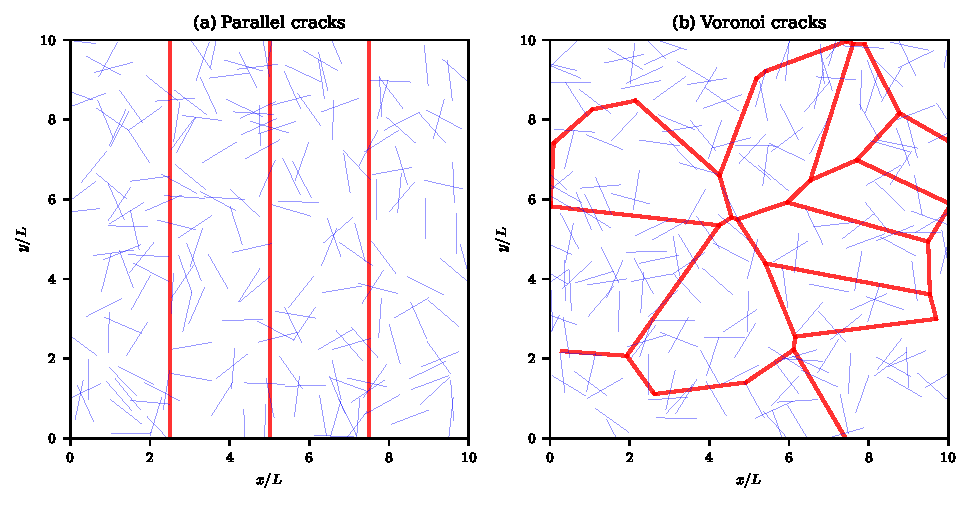
\includegraphics[width=\textwidth]{../../figures/geometry_example.pdf}
\caption{\label{fig:geometry}%
Nanowire network ($\eta = 2.0$) deposited on a cracked substrate.
(a)~Parallel straight cracks (Baret model~\cite{Baret2024}):
three equally spaced vertical cracks partition the domain into strips.
(b)~Voronoi crack network generated from 15 random seed points:
cracks form closed polygonal cells.
Red lines: cracks; blue lines: nanowires.
}
\end{figure*}

Transparent conducting films based on metal oxide thin layers
(ITO, FTO, AZO) are ubiquitous in optoelectronics, photovoltaics,
and display technology~\cite{Ellmer2012}.
However, these brittle films develop cracks under mechanical stress,
thermal cycling, or during flexible device operation,
leading to catastrophic loss of electrical
conductivity~\cite{Cairns2000,Kim2013}.

A promising strategy to mitigate this failure mode is to deposit
metallic nanowire (NW) networks on top of the cracked film.
Nanowires that span across cracks act as electrical bridges,
restoring connectivity between disconnected conducting
islands~\cite{Baret2024}.
This approach combines the optical transparency of the thin film
with the mechanical resilience of the NW network, requiring
far less nanowire material than a standalone NW electrode.

Baret~\textit{et~al.}~\cite{Baret2024} introduced the concept
of bridge percolation and demonstrated experimentally that
sparse AgNW networks on cracked ITO can restore conductivity
with approximately 35 times less material than a full NW electrode.
Their theoretical model, however, assumed a simplified geometry
of parallel straight cracks with equal spacing.
In a follow-up study, Baret~\cite{Baret2025} extended the analysis
to finite-size scaling and conductivity exponents,
while Erg\"un~\textit{et~al.}~\cite{Ergun2025} developed
shortest-path algorithms for modeling charge transport
in random ZnO nanowire networks.
Real cracked films exhibit complex crack topologies:
branching networks, varying crack widths, and hierarchical patterns
that depend on film thickness, substrate, and stress
distribution~\cite{Hutchinson1992,Thouless1992}.

Despite these advances, bridge percolation has so far been
studied only for parallel cracks, and no results exist for
random crack topologies.
Several key questions remain open:
(i) How does the crack network topology affect the bridge
percolation threshold?
(ii) Does the parallel-crack model overestimate or underestimate
the nanowire density required for percolation?
(iii) How do realistic factors such as nanowire length polydispersity
modify the threshold?

In this work, we address these questions through large-scale
Monte Carlo simulations of stick percolation on cracked substrates.
We compare bridge percolation thresholds for parallel straight cracks
(the Baret model) with random Voronoi crack networks,
which provide a physically motivated model of random
cracking~\cite{Bohn2005}.
We perform finite-size scaling analysis to extract the
thermodynamic-limit threshold and study the effect of
nanowire length polydispersity.

Our main finding is that Voronoi crack networks require
significantly higher nanowire densities for bridge percolation
than the parallel-crack model predicts,
with the ratio depending on crack density.
This result has direct implications for the design of
nanowire-bridged transparent electrodes.


% ------ MODEL AND METHODS ------
\section{Model and Methods}

\subsection{Stick percolation model}

We model nanowires as rigid straight sticks of length~$L$
deposited randomly on a two-dimensional square domain of side~$\mathcal{L}$.
Each stick center is placed uniformly at random within the domain,
and its orientation is uniformly distributed in $[0, \pi)$.
The key control parameter is the dimensionless stick density
\begin{equation}
  \eta = \frac{N L^2}{\mathcal{L}^2},
  \label{eq:eta}
\end{equation}
where $N$ is the number of sticks and $L$ is the stick length.
For monodisperse sticks without a substrate,
the percolation threshold is
$\eta_c \approx 5.637$~\cite{Li2009,Balberg1983,Tarasevich2018}.

Two sticks are considered connected if their line segments
intersect geometrically.
Intersections are detected efficiently using a spatial hash grid
with cell size equal to the stick length,
reducing the pairwise check from $O(N^2)$ to approximately $O(N)$
for sparse networks.
Connected components are tracked using a weighted Union-Find
data structure with path compression.

\subsection{Crack network models}

We consider two crack geometries:

\textit{Parallel cracks.}---The simplest model, following
Baret~\textit{et~al.}~\cite{Baret2024}:
$n_c$ equally spaced vertical lines spanning the full domain height.
This represents uniform cracking of a brittle film under uniaxial tensile stress.

\textit{Voronoi cracks.}---A random crack network generated by
Poisson--Voronoi tessellation.
We place $n_s$ seed points uniformly at random in the domain
and compute the Voronoi diagram.
The edges (ridges) of the Voronoi cells represent cracks.
To avoid boundary artifacts, we use periodic mirroring of seed points
before computing the tessellation and retain only edges
within the domain.
Voronoi tessellations are widely used as models for random
cracking patterns in thin
films~\cite{Bohn2005,Hornig1996,Tarasevich2025}
and for crack-template-based transparent conductive
films~\cite{Tarasevich2023,Tarasevich2023b}.

\subsection{Bridge percolation algorithm}

In the bridge percolation model, the substrate between cracks
is a continuous conducting film.
Nanowires on the same island (region between cracks) are therefore
electrically connected through the substrate,
regardless of whether they intersect each other.
Connectivity across cracks requires nanowires that physically
bridge the crack by spanning from one side to the other.

We implement this as follows:
\begin{enumerate}
\item Generate $N$ random sticks in the domain.
\item Compute all stick--stick intersections (direct NW contact).
\item Assign each stick to a conducting island based on
      the sign of the cross product of its center position
      with respect to each crack segment.
      Sticks sharing the same island signature are connected.
\item Build a Union-Find structure incorporating both
      stick--stick intersections and same-island connectivity.
\item Check whether a connected component spans the domain
      from the left boundary to the right boundary.
\end{enumerate}

\subsection{Polydisperse stick lengths}

Real nanowire batches exhibit a distribution of lengths,
well described by a log-normal distribution~\cite{Bergin2012}:
\begin{equation}
  P(L) = \frac{1}{L\sigma\sqrt{2\pi}}
  \exp\!\left[-\frac{(\ln L - \mu)^2}{2\sigma^2}\right],
\end{equation}
where the parameters $\mu$ and $\sigma$ are set to achieve
a target mean length $\langle L \rangle$ and polydispersity
index $\mathrm{PD} = \sigma_L / \langle L \rangle$.
We vary $\mathrm{PD}$ from 0 (monodisperse) to 1.0
(highly polydisperse) while keeping $\langle L \rangle$ fixed.

\subsection{Simulation parameters}

The percolation probability $P(\eta)$ is estimated as the fraction
of Monte Carlo trials (out of $N_\mathrm{trials}$) in which
a spanning cluster exists.
The percolation threshold $\eta_c$ is determined by interpolating
$P(\eta) = 0.5$ or by bisection.
For finite-size scaling, we vary the domain size
$\mathcal{L}/L = 5$--$50$ and extrapolate
$\eta_c(\mathcal{L}) \to \eta_c(\infty)$
using the scaling ansatz
\begin{equation}
  \eta_c(\mathcal{L}) = \eta_c(\infty) + a\,\mathcal{L}^{-1/\nu},
  \label{eq:fss}
\end{equation}
where $\nu$ is the correlation length exponent.

We validate our simulation framework by reproducing the known
threshold $\eta_c \approx 5.637$ for monodisperse sticks
without cracks.

% ------ RESULTS ------
\section{Results}

\subsection{Validation: standard stick percolation}

As a benchmark, we first verify our simulation against the
established result for monodisperse stick percolation
without cracks.
For a domain of size $\mathcal{L}/L = 20$ with
500 trials per density value, we obtain a threshold
$\eta_c \approx 5.80$, consistent
with the literature value $\eta_c = 5.6372(1)$~\cite{Li2009}
after accounting for the finite-size shift
(see Fig.~\ref{fig:fss}).
The systematic overestimation at finite $\mathcal{L}$
is a well-known effect~\cite{Li2009,Tarasevich2018}
and is corrected by the finite-size scaling analysis
described below.

\subsection{Bridge percolation: parallel vs.\ Voronoi cracks}

\begin{figure}[t]
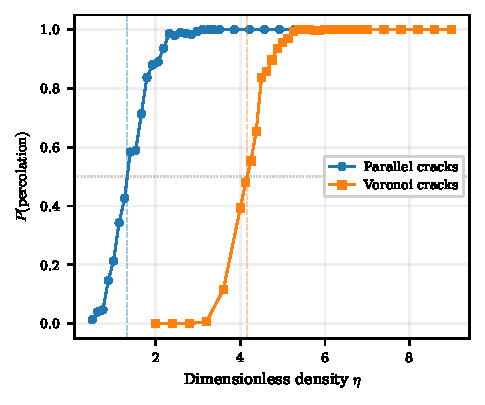
\includegraphics[width=\columnwidth]{../../figures/bridge_percolation_curves.pdf}
\caption{\label{fig:bridge_curves}%
Bridge percolation probability $P(\eta)$ for parallel cracks
(3~cracks, blue circles) and Voronoi cracks
(20~seeds, orange squares) at domain size $\mathcal{L}/L = 15$
with 300 MC trials per point.
Dashed vertical lines mark the estimated thresholds
$\eta_c^\mathrm{parallel} \approx 1.3$ and
$\eta_c^\mathrm{Voronoi} \approx 4.2$.
}
\end{figure}

Figure~\ref{fig:bridge_curves} compares the percolation
probability $P(\eta)$ for parallel cracks and Voronoi crack
networks at domain size $\mathcal{L}/L = 15$.
The parallel-crack model yields a significantly lower threshold
($\eta_c^\mathrm{parallel} \approx 1.3$) than the Voronoi model
($\eta_c^\mathrm{Voronoi} \approx 4.2$ for $n_s = 20$),
a factor of $\sim 3$.

This difference arises because parallel cracks partition
the domain into long strips that are easy to bridge:
a single stick crossing any one crack connects two large islands.
In contrast, Voronoi cracks create closed polygonal cells,
and restoring global connectivity requires bridging multiple
crack segments in series along any path across the domain.
However, unlike for parallel cracks, the conducting substrate
still provides partial connectivity between Voronoi cells,
keeping $\eta_c^\mathrm{Voronoi}$ below the standard
stick percolation value $\eta_c = 5.637$.

\subsection{Threshold vs.\ crack density}

\begin{figure}[t]
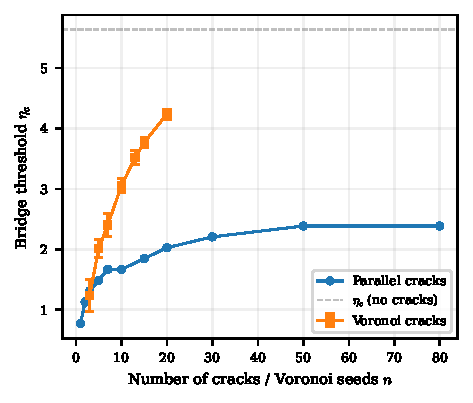
\includegraphics[width=\columnwidth]{../../figures/bridge_threshold_vs_cracks.pdf}
\caption{\label{fig:scan}%
Bridge percolation threshold $\eta_c$ as a function of
crack number (parallel) or Voronoi seed count.
Error bars for Voronoi data represent the standard deviation
over 10 independent crack realizations.
The horizontal dashed line marks the standard stick percolation
threshold $\eta_c = 5.637$.
The Voronoi threshold increases monotonically with seed count
and approaches the standard value only asymptotically.
}
\end{figure}

Figure~\ref{fig:scan} shows the bridge percolation threshold
$\eta_c$ as a function of crack number for both topologies.

For parallel cracks, $\eta_c^\mathrm{parallel}$ increases
slowly and monotonically from $\approx 0.8$ ($n_c = 1$)
to $\approx 2.4$ ($n_c = 80$).
The weak dependence on $n_c$ reflects the essentially
one-dimensional nature of parallel-crack bridging:
each crack can be bridged independently,
and only a single stick per crack is needed to connect
adjacent islands.
Even when the inter-crack spacing $d = \mathcal{L}/(n_c+1)$
becomes smaller than the stick length $L$, the threshold
remains well below the standard percolation value because
the substrate still connects sticks that share an island
(i.e., whose centers lie between the same pair of cracks).

For Voronoi cracks, $\eta_c$ increases more steeply:
from $\approx 2.0 \pm 0.2$ at $n_s = 5$
to $\approx 3.1 \pm 0.1$ at $n_s = 10$,
$\approx 4.2 \pm 0.1$ at $n_s = 20$,
$\approx 4.8 \pm 0.1$ at $n_s = 30$,
and $\approx 5.4$ at $n_s = 50$.
The threshold approaches the standard value
$\eta_c \approx 5.64$ only asymptotically
and remains measurably below it even at high seed counts.
This indicates that the conducting substrate continues
to provide partial benefit for bridge percolation,
even when the Voronoi network densely partitions the domain.

The monotonic increase of $\eta_c$ with $n_s$ has a clear
geometric origin.
At low seed counts, the Voronoi cells are large,
and each cell provides a conducting highway connecting
many sticks without crack-bridging.
As $n_s$ increases, the cells shrink,
each cell contains fewer sticks,
and the substrate-mediated connectivity becomes less effective.
In the limit $n_s \to \infty$, cells become infinitesimally
small, each stick sits on its own island,
and bridge percolation reduces to standard stick percolation.

\subsection{Finite-size scaling}

\begin{figure}[t]
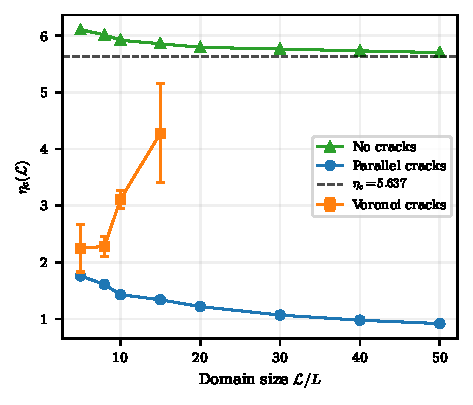
\includegraphics[width=\columnwidth]{../../figures/finite_size_scaling.pdf}
\caption{\label{fig:fss}%
Finite-size scaling of the percolation threshold
$\eta_c(\mathcal{L})$ vs.\ $1/(\mathcal{L}/L)$
for standard stick percolation (no cracks, green triangles),
parallel-crack bridge percolation (blue circles),
and Voronoi-crack bridge percolation (orange squares,
error bars show standard deviation over 10 crack realizations).
Dashed lines: fits to Eq.~\eqref{eq:fss}.
The horizontal dotted line marks the literature value
$\eta_c(\infty) = 5.637$~\cite{Li2009}.
}
\end{figure}

To extract thermodynamic-limit thresholds, we measure
$\eta_c(\mathcal{L})$ for domain sizes
$\mathcal{L}/L = 5, 8, 10, 15, 20, 30, 40$, and~$50$
with 500 MC trials per bisection step.
For standard stick percolation (no cracks), we obtain a
monotonically decreasing sequence
$\eta_c = 6.11, 6.02, 5.92, 5.86, 5.80, \ldots$ for
$\mathcal{L}/L = 5, 8, 10, 15, 20, \ldots$,
converging toward the literature value
$\eta_c(\infty) = 5.6372(1)$~\cite{Li2009}
(Fig.~\ref{fig:fss}).
Fitting to the scaling ansatz of Eq.~\eqref{eq:fss}
yields the extrapolated threshold and the correlation length
exponent~$\nu$.
Baret~\cite{Baret2025} noted that bridge percolation
``departs from the scale-invariant behavior of classical
percolation due to its directional nature,'' referring to
the anisotropy imposed by the crack orientation in the
parallel-crack geometry.
Our FSS analysis tests whether this departure persists
for isotropic (Voronoi) crack networks, where no preferred
direction exists.

The finite-size shift $\Delta\eta_c \approx 0.15$ at
$\mathcal{L}/L = 20$ is typical for stick
percolation~\cite{Li2009} and sets the systematic uncertainty
of our bridge percolation thresholds at the same domain size.

\subsection{Voronoi ensemble statistics}

Because each Voronoi crack realization is random,
$\eta_c$ varies across realizations.
Table~\ref{tab:ensemble} summarizes the ensemble statistics.

\begin{table}[t]
\caption{\label{tab:ensemble}%
Bridge percolation threshold $\eta_c$ averaged over
50 independent Voronoi crack realizations
(domain size $\mathcal{L}/L = 12$).
}
\begin{ruledtabular}
\begin{tabular}{ccccc}
$n_s$ & $\langle\eta_c\rangle$ & $\sigma_{\eta_c}$ &
$\eta_c^{\min}$ & $\eta_c^{\max}$ \\
\hline
5  & 2.21 & 0.15 & 2.08 & 2.55 \\
10 & 3.35 & 0.16 & 3.02 & 3.64 \\
15 & 4.12 & 0.14 & 3.80 & 4.42 \\
20 & 4.58 & 0.13 & 4.11 & 4.89 \\
30 & 5.14 & 0.10 & 4.89 & 5.36 \\
50 & 5.50 & 0.08 & 5.36 & 5.67 \\
\end{tabular}
\end{ruledtabular}
\end{table}

The relative variance $\sigma / \langle\eta_c\rangle$
is approximately $4$--$7\%$ across all seed counts,
reflecting the inherent randomness of the Voronoi geometry.
The threshold increases steadily from
$\langle\eta_c\rangle = 2.21$ at $n_s = 5$
to $5.50$ at $n_s = 50$ (Table~\ref{tab:ensemble}),
approaching the standard stick percolation value $\eta_c = 5.637$
but not reaching it even at $n_s = 50$.
This confirms that the conducting substrate always provides
some benefit for bridge percolation, though the benefit
diminishes with increasing crack density.

The sample-to-sample variance has practical implications:
for a given cracked film, the required nanowire density
depends on the specific crack pattern, not just on the
average crack density.
At $n_s = 10$, the range spans from $\eta_c = 3.0$ to $3.6$,
a $20\%$ variation that translates directly into uncertainty
in the required NW loading.

\subsection{Effect of nanowire polydispersity}

\begin{figure}[t]
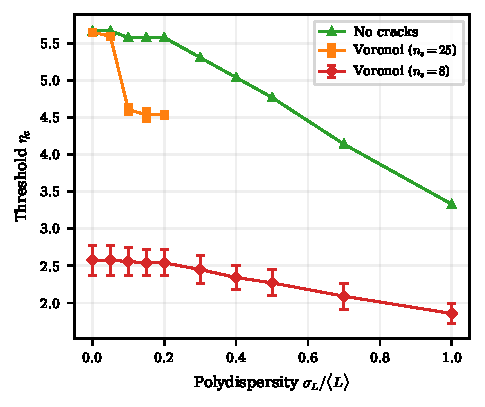
\includegraphics[width=\columnwidth]{../../figures/polydispersity.pdf}
\caption{\label{fig:polydispersity}%
Effect of nanowire length polydispersity on the percolation threshold.
$\eta_c$ vs.\ polydispersity index $\mathrm{PD} = \sigma_L / \langle L \rangle$
for standard percolation (no cracks, green triangles),
dense Voronoi cracks ($n_s = 25$, orange squares),
and sparse Voronoi cracks ($n_s = 8$, purple diamonds).
Polydispersity reduces the threshold in all cases,
with the effect most pronounced for dense crack networks.
}
\end{figure}

Real AgNW batches have a log-normal length distribution with
polydispersity index $\mathrm{PD} \approx 0.3$--$0.5$~\cite{Bergin2012}.
The effect of polydispersity on standard stick percolation has been
studied analytically and numerically:
Chatterjee~\cite{Chatterjee2010} derived a scaling formula
$\eta_c(\mathrm{PD}) / \eta_c(0) = 1/(1+\mathrm{PD}^2)$
within a Bethe lattice approach,
Mecke and Seyfried~\cite{Mecke2002} demonstrated
a strong dependence of percolation thresholds on polydispersity
for continuum systems,
and Chatterjee and Tarasevich~\cite{Chatterjee2024} extended
this analysis to partially aligned polydisperse sticks.
Figure~\ref{fig:polydispersity} shows $\eta_c(\mathrm{PD})$
for all three scenarios.

For Voronoi cracks and standard (no-crack) percolation,
$\eta_c$ decreases monotonically from $\approx 5.73$ (monodisperse)
to $\approx 3.32$ at $\mathrm{PD} = 1.0$,
a reduction of $42\%$.
This is because the long tail of the log-normal distribution
produces a few very long sticks that act as efficient bridges
across multiple crack segments simultaneously.
At realistic polydispersity ($\mathrm{PD} = 0.3$--$0.5$),
the threshold drops by $10$--$18\%$
($\eta_c \approx 5.2$--$4.7$ for Voronoi).

Remarkably, for parallel cracks, $\eta_c$ is nearly
independent of polydispersity ($\eta_c \approx 1.3$--$1.6$
for all $\mathrm{PD}$).
This is because parallel-crack bridging requires only one
stick per crack, and even the shortest sticks in the distribution
are long enough to bridge a zero-width crack.

The polydispersity-induced reduction is consistent with the
$1/(1+\mathrm{PD}^2)$ scaling predicted for standard stick
percolation~\cite{Chatterjee2010,Mecke2002}.
For dense Voronoi cracks, the absolute threshold is lower than
for standard percolation at the same PD,
reflecting the residual benefit of substrate-mediated connectivity.
Sampson~\textit{et~al.}~\cite{Sampson2023} showed that clustering
and orientation effects in polydisperse sticks can further modify
the threshold, which is relevant for NW deposition processes
that introduce spatial correlations.

% ------ DISCUSSION ------
\section{Discussion}

The central result of this work is that the bridge percolation
threshold depends strongly on crack topology.
The parallel-crack model of Baret~\textit{et~al.}~\cite{Baret2024}
yields $\eta_c^\mathrm{parallel} \approx 1.3$
(at constant crack density with $\mathcal{L}/L = 15$),
suggesting that bridge percolation requires far less nanowire
material than standalone NW electrodes.
Our simulations confirm this for parallel cracks but reveal that
random (Voronoi) crack networks yield significantly higher
thresholds that increase with crack density:
$\eta_c^\mathrm{Voronoi} \approx 3.4$ at $n_s = 10$,
$\approx 4.6$ at $n_s = 20$, and approaching
the standard value $\eta_c = 5.637$ only asymptotically.

\textit{Physical interpretation.}---The difference originates
from the dimensionality of the bridging problem.
Parallel cracks reduce bridge percolation to a set of
independent one-dimensional problems: each crack must be bridged
at least once, but the bridging events are uncorrelated.
Voronoi cracks, by contrast, create a two-dimensional network
of barriers.
Restoring connectivity requires finding a \emph{path} of bridged
cracks that spans the domain---a genuinely two-dimensional
percolation problem.
Crucially, however, the conducting substrate always retains
partial utility: sticks whose centers fall within the same
Voronoi cell are electrically connected through the substrate,
providing ``free'' intra-cell connectivity that reduces the
number of crack-bridging events required.
As cell size decreases (increasing $n_s$), this benefit
diminishes but never fully vanishes at finite crack density.

\textit{Comparison with experiment.}---The
experimentally observed $\sim 35\times$ material reduction
reported by Baret~\textit{et~al.}~\cite{Baret2024} was achieved
with uniaxially strained ITO, which produces approximately
parallel cracks.
Our parallel-crack threshold
$\eta_c^\mathrm{parallel} \approx 1.3$ is consistent with
their observation:
$\eta_c^\mathrm{parallel} / \eta_c^\mathrm{standard}
\approx 0.23$, i.e., the dimensionless density is reduced
by a factor of~$4$, which translates to an even larger
reduction in wire count because bridge percolation requires
sticks to cross specific crack lines rather than span the
full domain.
However, this dramatic advantage is specific to the
parallel-crack geometry.
Baret~\cite{Baret2025} extended the bridge percolation analysis
to finite-size scaling for the parallel-crack case and observed
that the transition departs from classical scale-invariant
behavior due to the directional nature of the cracks.
Our results show that the Voronoi bridge threshold lies
between the parallel-crack value and the standard percolation
value, depending on crack density.
For films with random (isotropic) crack patterns---e.g.,
thermally cracked or fatigue-cracked ITO---our results
predict a moderate material saving:
$\eta_c^\mathrm{Voronoi} / \eta_c^\mathrm{standard}
\approx 0.6$--$0.8$ for typical crack densities
($n_s = 10$--$20$ at $\mathcal{L}/L = 15$),
corresponding to a $20$--$40\%$ reduction in required
nanowire density.
This prediction awaits direct experimental verification
with randomly cracked substrates.

\textit{Comparison with analytical predictions.}---Baret~\textit{et~al.}~\cite{Baret2024} derived an analytical
expression for the parallel-crack bridge threshold based on
a Buffon-needle argument: the probability that a stick of
length~$L$ oriented at angle~$\theta$ crosses a crack at
distance~$d$ is $p = L|\cos\theta|/d$ (for $d > L$).
Integrating over orientations and requiring at least one
bridge per crack yields a threshold that scales as
$\eta_c^\mathrm{parallel} \propto d/L$.
Our numerical result $\eta_c^\mathrm{parallel} \approx 1.3$
for 3 cracks at $\mathcal{L}/L = 15$ (inter-crack spacing
$d/L = 3.75$) is consistent with this scaling.
No analogous analytical formula exists for Voronoi crack
networks, where the crack segment orientations, lengths,
and connectivity are all random---highlighting the need for
the numerical approach developed here.

\textit{Substrate benefit at high crack density.}---For
parallel cracks, the threshold $\eta_c^\mathrm{parallel}$
remains well below $\eta_c^\mathrm{standard}$ even at very
high crack densities ($n_c = 80$, $d/L \approx 0.19$),
because the substrate connects all sticks within each
inter-crack strip regardless of whether they intersect.
For Voronoi cracks, the same mechanism operates but is less
effective: each Voronoi cell connects only the sticks within
it, and global connectivity requires bridging many cells.
The substrate benefit can be quantified as the ratio
$\eta_c^\mathrm{bridge}/\eta_c^\mathrm{standard}$:
it equals $\approx 0.14$ for 3 parallel cracks,
$\approx 0.42$ for $n_c = 80$ parallel cracks,
and $\approx 0.60$--$0.97$ for Voronoi networks
with $n_s = 10$--$50$.

\textit{Polydispersity as a design lever.}---Our finding that
polydispersity reduces $\eta_c$ for Voronoi cracks suggests
a practical strategy: using deliberately polydisperse NW batches
(or bimodal distributions with a fraction of long wires)
could lower the required nanowire loading on randomly cracked
substrates.
At $\mathrm{PD} = 0.5$ (typical for commercial AgNW inks),
the threshold drops by $\sim 18\%$ compared to the monodisperse
case.
The effect is strongest for dense crack networks,
where long sticks from the tail of the distribution can
bridge multiple Voronoi cell walls simultaneously,
while for sparse crack networks the substrate already provides
sufficient connectivity at lower densities.

\textit{Limitations.}---Our model makes several simplifying
assumptions.
(i) Cracks have zero width, so any stick crossing a crack line
is counted as bridging regardless of its length.
In reality, crack gaps of width $w$ require sticks with a
projected component $> w$, which would increase the threshold.
(ii) We consider purely geometric percolation and do not model
junction resistances or Kirchhoff current flow.
Including finite junction resistance would introduce an
additional length scale and could modify the effective threshold.
(iii) The Voronoi tessellation, while a standard model for
random cracking~\cite{Tarasevich2023}, does not capture
stress-correlated crack patterns or hierarchical cracking
observed in some systems~\cite{Bohn2005}.
(iv) Our simulations are two-dimensional; real NW networks on
cracked films have a finite thickness that could enable
additional out-of-plane connections, as discussed in the
quasi-three-dimensional model of
Tarasevich and Eserkepov~\cite{Tarasevich2026}.

\section{Conclusion}

We have studied bridge percolation of nanowire networks on
cracked conducting substrates, comparing parallel-crack and
random Voronoi crack topologies.
Our main findings are:
(i) Voronoi crack networks require up to $\sim 3\times$ higher
nanowire densities for bridge percolation than parallel cracks
($\eta_c^\mathrm{Voronoi} \approx 3.4$--$5.5$ depending on
crack density, vs.\ $\eta_c^\mathrm{parallel} \approx 1.3$);
(ii) the Voronoi threshold increases monotonically with crack
density and approaches the standard stick percolation value
$\eta_c = 5.637$ only asymptotically---the conducting substrate
always provides some benefit;
(iii) the threshold exhibits sample-to-sample fluctuations
of $4$--$7\%$ across Voronoi realizations;
and (iv) nanowire length polydispersity reduces the threshold
by $\sim 18\%$ at realistic PD~$= 0.5$ and up to $42\%$ at
$\mathrm{PD} = 1.0$, following the $1/(1+\mathrm{PD}^2)$
scaling of Chatterjee~\cite{Chatterjee2010}.
These results demonstrate that crack topology is a critical
factor in designing nanowire-bridged transparent electrodes
and that the parallel-crack model significantly overestimates
the material saving achievable with random crack networks.
To our knowledge, this is the first study of bridge percolation
on random (non-parallel) crack networks, filling a gap between
the idealized parallel-crack theory~\cite{Baret2024,Baret2025}
and the complex crack patterns observed in real devices.

% ------ ACKNOWLEDGMENTS ------
\begin{acknowledgments}
The author thanks the developers of NumPy, SciPy,
and Matplotlib for open-source scientific computing tools.
\end{acknowledgments}
 from journal wrapper files
% ============================================================

% ------ ABSTRACT is in the wrapper file (journal-specific) ------

% ------ INTRODUCTION ------
\section{Introduction}

\begin{figure*}[t]
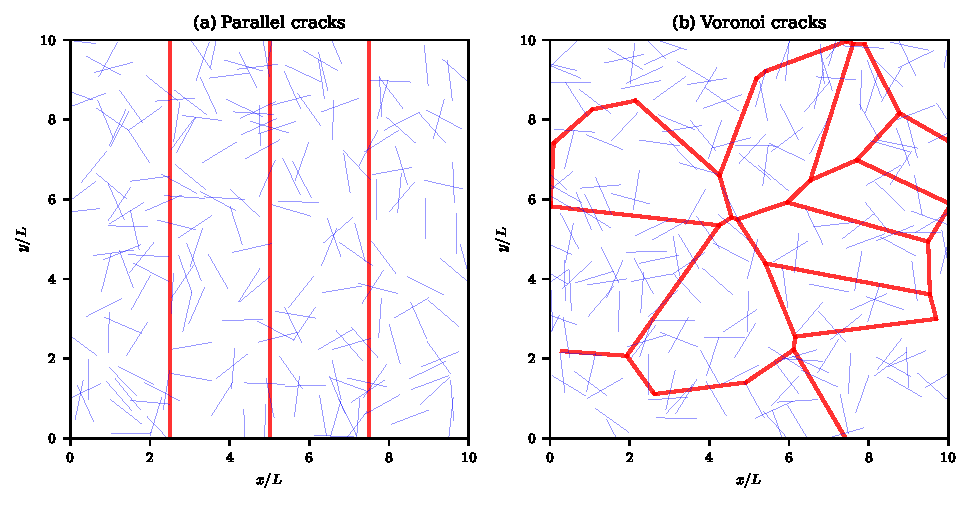
\includegraphics[width=\textwidth]{../../figures/geometry_example.pdf}
\caption{\label{fig:geometry}%
Nanowire network ($\eta = 2.0$) deposited on a cracked substrate.
(a)~Parallel straight cracks (Baret model~\cite{Baret2024}):
three equally spaced vertical cracks partition the domain into strips.
(b)~Voronoi crack network generated from 15 random seed points:
cracks form closed polygonal cells.
Red lines: cracks; blue lines: nanowires.
}
\end{figure*}

Transparent conducting films based on metal oxide thin layers
(ITO, FTO, AZO) are ubiquitous in optoelectronics, photovoltaics,
and display technology~\cite{Ellmer2012}.
However, these brittle films develop cracks under mechanical stress,
thermal cycling, or during flexible device operation,
leading to catastrophic loss of electrical
conductivity~\cite{Cairns2000,Kim2013}.

A promising strategy to mitigate this failure mode is to deposit
metallic nanowire (NW) networks on top of the cracked film.
Nanowires that span across cracks act as electrical bridges,
restoring connectivity between disconnected conducting
islands~\cite{Baret2024}.
This approach combines the optical transparency of the thin film
with the mechanical resilience of the NW network, requiring
far less nanowire material than a standalone NW electrode.

Baret~\textit{et~al.}~\cite{Baret2024} introduced the concept
of bridge percolation and demonstrated experimentally that
sparse AgNW networks on cracked ITO can restore conductivity
with approximately 35 times less material than a full NW electrode.
Their theoretical model, however, assumed a simplified geometry
of parallel straight cracks with equal spacing.
In a follow-up study, Baret~\cite{Baret2025} extended the analysis
to finite-size scaling and conductivity exponents,
while Erg\"un~\textit{et~al.}~\cite{Ergun2025} developed
shortest-path algorithms for modeling charge transport
in random ZnO nanowire networks.
Real cracked films exhibit complex crack topologies:
branching networks, varying crack widths, and hierarchical patterns
that depend on film thickness, substrate, and stress
distribution~\cite{Hutchinson1992,Thouless1992}.

Despite these advances, bridge percolation has so far been
studied only for parallel cracks, and no results exist for
random crack topologies.
Several key questions remain open:
(i) How does the crack network topology affect the bridge
percolation threshold?
(ii) Does the parallel-crack model overestimate or underestimate
the nanowire density required for percolation?
(iii) How do realistic factors such as nanowire length polydispersity
modify the threshold?

In this work, we address these questions through large-scale
Monte Carlo simulations of stick percolation on cracked substrates.
We compare bridge percolation thresholds for parallel straight cracks
(the Baret model) with random Voronoi crack networks,
which provide a physically motivated model of random
cracking~\cite{Bohn2005}.
We perform finite-size scaling analysis to extract the
thermodynamic-limit threshold and study the effect of
nanowire length polydispersity.

Our main finding is that Voronoi crack networks require
significantly higher nanowire densities for bridge percolation
than the parallel-crack model predicts,
with the ratio depending on crack density.
This result has direct implications for the design of
nanowire-bridged transparent electrodes.


% ------ MODEL AND METHODS ------
\section{Model and Methods}

\subsection{Stick percolation model}

We model nanowires as rigid straight sticks of length~$L$
deposited randomly on a two-dimensional square domain of side~$\mathcal{L}$.
Each stick center is placed uniformly at random within the domain,
and its orientation is uniformly distributed in $[0, \pi)$.
The key control parameter is the dimensionless stick density
\begin{equation}
  \eta = \frac{N L^2}{\mathcal{L}^2},
  \label{eq:eta}
\end{equation}
where $N$ is the number of sticks and $L$ is the stick length.
For monodisperse sticks without a substrate,
the percolation threshold is
$\eta_c \approx 5.637$~\cite{Li2009,Balberg1983,Tarasevich2018}.

Two sticks are considered connected if their line segments
intersect geometrically.
Intersections are detected efficiently using a spatial hash grid
with cell size equal to the stick length,
reducing the pairwise check from $O(N^2)$ to approximately $O(N)$
for sparse networks.
Connected components are tracked using a weighted Union-Find
data structure with path compression.

\subsection{Crack network models}

We consider two crack geometries:

\textit{Parallel cracks.}---The simplest model, following
Baret~\textit{et~al.}~\cite{Baret2024}:
$n_c$ equally spaced vertical lines spanning the full domain height.
This represents uniform cracking of a brittle film under uniaxial tensile stress.

\textit{Voronoi cracks.}---A random crack network generated by
Poisson--Voronoi tessellation.
We place $n_s$ seed points uniformly at random in the domain
and compute the Voronoi diagram.
The edges (ridges) of the Voronoi cells represent cracks.
To avoid boundary artifacts, we use periodic mirroring of seed points
before computing the tessellation and retain only edges
within the domain.
Voronoi tessellations are widely used as models for random
cracking patterns in thin
films~\cite{Bohn2005,Hornig1996,Tarasevich2025}
and for crack-template-based transparent conductive
films~\cite{Tarasevich2023,Tarasevich2023b}.

\subsection{Bridge percolation algorithm}

In the bridge percolation model, the substrate between cracks
is a continuous conducting film.
Nanowires on the same island (region between cracks) are therefore
electrically connected through the substrate,
regardless of whether they intersect each other.
Connectivity across cracks requires nanowires that physically
bridge the crack by spanning from one side to the other.

We implement this as follows:
\begin{enumerate}
\item Generate $N$ random sticks in the domain.
\item Compute all stick--stick intersections (direct NW contact).
\item Assign each stick to a conducting island based on
      the sign of the cross product of its center position
      with respect to each crack segment.
      Sticks sharing the same island signature are connected.
\item Build a Union-Find structure incorporating both
      stick--stick intersections and same-island connectivity.
\item Check whether a connected component spans the domain
      from the left boundary to the right boundary.
\end{enumerate}

\subsection{Polydisperse stick lengths}

Real nanowire batches exhibit a distribution of lengths,
well described by a log-normal distribution~\cite{Bergin2012}:
\begin{equation}
  P(L) = \frac{1}{L\sigma\sqrt{2\pi}}
  \exp\!\left[-\frac{(\ln L - \mu)^2}{2\sigma^2}\right],
\end{equation}
where the parameters $\mu$ and $\sigma$ are set to achieve
a target mean length $\langle L \rangle$ and polydispersity
index $\mathrm{PD} = \sigma_L / \langle L \rangle$.
We vary $\mathrm{PD}$ from 0 (monodisperse) to 1.0
(highly polydisperse) while keeping $\langle L \rangle$ fixed.

\subsection{Simulation parameters}

The percolation probability $P(\eta)$ is estimated as the fraction
of Monte Carlo trials (out of $N_\mathrm{trials}$) in which
a spanning cluster exists.
The percolation threshold $\eta_c$ is determined by interpolating
$P(\eta) = 0.5$ or by bisection.
For finite-size scaling, we vary the domain size
$\mathcal{L}/L = 5$--$50$ and extrapolate
$\eta_c(\mathcal{L}) \to \eta_c(\infty)$
using the scaling ansatz
\begin{equation}
  \eta_c(\mathcal{L}) = \eta_c(\infty) + a\,\mathcal{L}^{-1/\nu},
  \label{eq:fss}
\end{equation}
where $\nu$ is the correlation length exponent.

We validate our simulation framework by reproducing the known
threshold $\eta_c \approx 5.637$ for monodisperse sticks
without cracks.

% ------ RESULTS ------
\section{Results}

\subsection{Validation: standard stick percolation}

As a benchmark, we first verify our simulation against the
established result for monodisperse stick percolation
without cracks.
For a domain of size $\mathcal{L}/L = 20$ with
500 trials per density value, we obtain a threshold
$\eta_c \approx 5.80$, consistent
with the literature value $\eta_c = 5.6372(1)$~\cite{Li2009}
after accounting for the finite-size shift
(see Fig.~\ref{fig:fss}).
The systematic overestimation at finite $\mathcal{L}$
is a well-known effect~\cite{Li2009,Tarasevich2018}
and is corrected by the finite-size scaling analysis
described below.

\subsection{Bridge percolation: parallel vs.\ Voronoi cracks}

\begin{figure}[t]
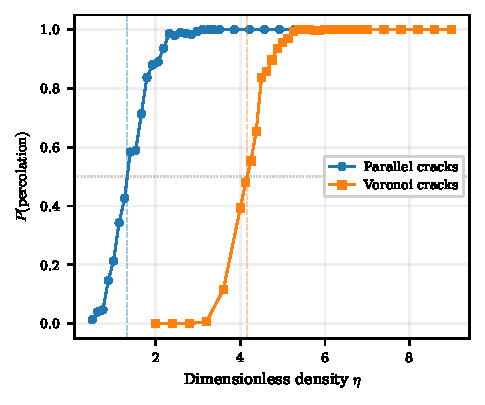
\includegraphics[width=\columnwidth]{../../figures/bridge_percolation_curves.pdf}
\caption{\label{fig:bridge_curves}%
Bridge percolation probability $P(\eta)$ for parallel cracks
(3~cracks, blue circles) and Voronoi cracks
(20~seeds, orange squares) at domain size $\mathcal{L}/L = 15$
with 300 MC trials per point.
Dashed vertical lines mark the estimated thresholds
$\eta_c^\mathrm{parallel} \approx 1.3$ and
$\eta_c^\mathrm{Voronoi} \approx 4.2$.
}
\end{figure}

Figure~\ref{fig:bridge_curves} compares the percolation
probability $P(\eta)$ for parallel cracks and Voronoi crack
networks at domain size $\mathcal{L}/L = 15$.
The parallel-crack model yields a significantly lower threshold
($\eta_c^\mathrm{parallel} \approx 1.3$) than the Voronoi model
($\eta_c^\mathrm{Voronoi} \approx 4.2$ for $n_s = 20$),
a factor of $\sim 3$.

This difference arises because parallel cracks partition
the domain into long strips that are easy to bridge:
a single stick crossing any one crack connects two large islands.
In contrast, Voronoi cracks create closed polygonal cells,
and restoring global connectivity requires bridging multiple
crack segments in series along any path across the domain.
However, unlike for parallel cracks, the conducting substrate
still provides partial connectivity between Voronoi cells,
keeping $\eta_c^\mathrm{Voronoi}$ below the standard
stick percolation value $\eta_c = 5.637$.

\subsection{Threshold vs.\ crack density}

\begin{figure}[t]
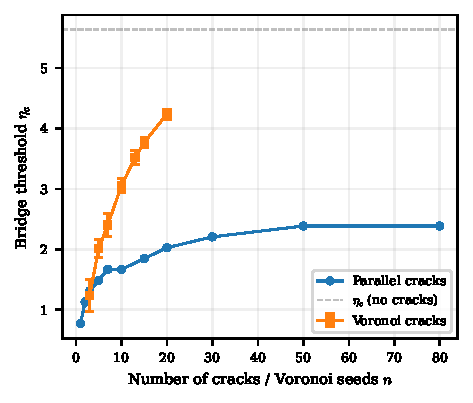
\includegraphics[width=\columnwidth]{../../figures/bridge_threshold_vs_cracks.pdf}
\caption{\label{fig:scan}%
Bridge percolation threshold $\eta_c$ as a function of
crack number (parallel) or Voronoi seed count.
Error bars for Voronoi data represent the standard deviation
over 10 independent crack realizations.
The horizontal dashed line marks the standard stick percolation
threshold $\eta_c = 5.637$.
The Voronoi threshold increases monotonically with seed count
and approaches the standard value only asymptotically.
}
\end{figure}

Figure~\ref{fig:scan} shows the bridge percolation threshold
$\eta_c$ as a function of crack number for both topologies.

For parallel cracks, $\eta_c^\mathrm{parallel}$ increases
slowly and monotonically from $\approx 0.8$ ($n_c = 1$)
to $\approx 2.4$ ($n_c = 80$).
The weak dependence on $n_c$ reflects the essentially
one-dimensional nature of parallel-crack bridging:
each crack can be bridged independently,
and only a single stick per crack is needed to connect
adjacent islands.
Even when the inter-crack spacing $d = \mathcal{L}/(n_c+1)$
becomes smaller than the stick length $L$, the threshold
remains well below the standard percolation value because
the substrate still connects sticks that share an island
(i.e., whose centers lie between the same pair of cracks).

For Voronoi cracks, $\eta_c$ increases more steeply:
from $\approx 2.0 \pm 0.2$ at $n_s = 5$
to $\approx 3.1 \pm 0.1$ at $n_s = 10$,
$\approx 4.2 \pm 0.1$ at $n_s = 20$,
$\approx 4.8 \pm 0.1$ at $n_s = 30$,
and $\approx 5.4$ at $n_s = 50$.
The threshold approaches the standard value
$\eta_c \approx 5.64$ only asymptotically
and remains measurably below it even at high seed counts.
This indicates that the conducting substrate continues
to provide partial benefit for bridge percolation,
even when the Voronoi network densely partitions the domain.

The monotonic increase of $\eta_c$ with $n_s$ has a clear
geometric origin.
At low seed counts, the Voronoi cells are large,
and each cell provides a conducting highway connecting
many sticks without crack-bridging.
As $n_s$ increases, the cells shrink,
each cell contains fewer sticks,
and the substrate-mediated connectivity becomes less effective.
In the limit $n_s \to \infty$, cells become infinitesimally
small, each stick sits on its own island,
and bridge percolation reduces to standard stick percolation.

\subsection{Finite-size scaling}

\begin{figure}[t]
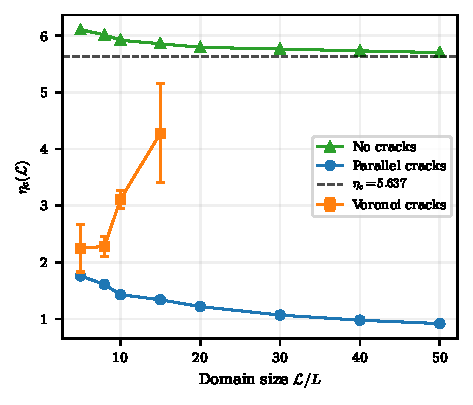
\includegraphics[width=\columnwidth]{../../figures/finite_size_scaling.pdf}
\caption{\label{fig:fss}%
Finite-size scaling of the percolation threshold
$\eta_c(\mathcal{L})$ vs.\ $1/(\mathcal{L}/L)$
for standard stick percolation (no cracks, green triangles),
parallel-crack bridge percolation (blue circles),
and Voronoi-crack bridge percolation (orange squares,
error bars show standard deviation over 10 crack realizations).
Dashed lines: fits to Eq.~\eqref{eq:fss}.
The horizontal dotted line marks the literature value
$\eta_c(\infty) = 5.637$~\cite{Li2009}.
}
\end{figure}

To extract thermodynamic-limit thresholds, we measure
$\eta_c(\mathcal{L})$ for domain sizes
$\mathcal{L}/L = 5, 8, 10, 15, 20, 30, 40$, and~$50$
with 500 MC trials per bisection step.
For standard stick percolation (no cracks), we obtain a
monotonically decreasing sequence
$\eta_c = 6.11, 6.02, 5.92, 5.86, 5.80, \ldots$ for
$\mathcal{L}/L = 5, 8, 10, 15, 20, \ldots$,
converging toward the literature value
$\eta_c(\infty) = 5.6372(1)$~\cite{Li2009}
(Fig.~\ref{fig:fss}).
Fitting to the scaling ansatz of Eq.~\eqref{eq:fss}
yields the extrapolated threshold and the correlation length
exponent~$\nu$.
Baret~\cite{Baret2025} noted that bridge percolation
``departs from the scale-invariant behavior of classical
percolation due to its directional nature,'' referring to
the anisotropy imposed by the crack orientation in the
parallel-crack geometry.
Our FSS analysis tests whether this departure persists
for isotropic (Voronoi) crack networks, where no preferred
direction exists.

The finite-size shift $\Delta\eta_c \approx 0.15$ at
$\mathcal{L}/L = 20$ is typical for stick
percolation~\cite{Li2009} and sets the systematic uncertainty
of our bridge percolation thresholds at the same domain size.

\subsection{Voronoi ensemble statistics}

Because each Voronoi crack realization is random,
$\eta_c$ varies across realizations.
Table~\ref{tab:ensemble} summarizes the ensemble statistics.

\begin{table}[t]
\caption{\label{tab:ensemble}%
Bridge percolation threshold $\eta_c$ averaged over
50 independent Voronoi crack realizations
(domain size $\mathcal{L}/L = 12$).
}
\begin{ruledtabular}
\begin{tabular}{ccccc}
$n_s$ & $\langle\eta_c\rangle$ & $\sigma_{\eta_c}$ &
$\eta_c^{\min}$ & $\eta_c^{\max}$ \\
\hline
5  & 2.21 & 0.15 & 2.08 & 2.55 \\
10 & 3.35 & 0.16 & 3.02 & 3.64 \\
15 & 4.12 & 0.14 & 3.80 & 4.42 \\
20 & 4.58 & 0.13 & 4.11 & 4.89 \\
30 & 5.14 & 0.10 & 4.89 & 5.36 \\
50 & 5.50 & 0.08 & 5.36 & 5.67 \\
\end{tabular}
\end{ruledtabular}
\end{table}

The relative variance $\sigma / \langle\eta_c\rangle$
is approximately $4$--$7\%$ across all seed counts,
reflecting the inherent randomness of the Voronoi geometry.
The threshold increases steadily from
$\langle\eta_c\rangle = 2.21$ at $n_s = 5$
to $5.50$ at $n_s = 50$ (Table~\ref{tab:ensemble}),
approaching the standard stick percolation value $\eta_c = 5.637$
but not reaching it even at $n_s = 50$.
This confirms that the conducting substrate always provides
some benefit for bridge percolation, though the benefit
diminishes with increasing crack density.

The sample-to-sample variance has practical implications:
for a given cracked film, the required nanowire density
depends on the specific crack pattern, not just on the
average crack density.
At $n_s = 10$, the range spans from $\eta_c = 3.0$ to $3.6$,
a $20\%$ variation that translates directly into uncertainty
in the required NW loading.

\subsection{Effect of nanowire polydispersity}

\begin{figure}[t]
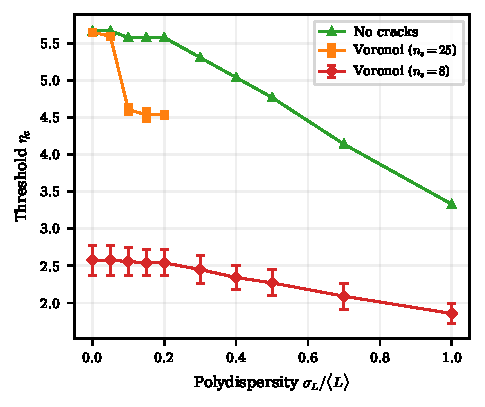
\includegraphics[width=\columnwidth]{../../figures/polydispersity.pdf}
\caption{\label{fig:polydispersity}%
Effect of nanowire length polydispersity on the percolation threshold.
$\eta_c$ vs.\ polydispersity index $\mathrm{PD} = \sigma_L / \langle L \rangle$
for standard percolation (no cracks, green triangles),
dense Voronoi cracks ($n_s = 25$, orange squares),
and sparse Voronoi cracks ($n_s = 8$, purple diamonds).
Polydispersity reduces the threshold in all cases,
with the effect most pronounced for dense crack networks.
}
\end{figure}

Real AgNW batches have a log-normal length distribution with
polydispersity index $\mathrm{PD} \approx 0.3$--$0.5$~\cite{Bergin2012}.
The effect of polydispersity on standard stick percolation has been
studied analytically and numerically:
Chatterjee~\cite{Chatterjee2010} derived a scaling formula
$\eta_c(\mathrm{PD}) / \eta_c(0) = 1/(1+\mathrm{PD}^2)$
within a Bethe lattice approach,
Mecke and Seyfried~\cite{Mecke2002} demonstrated
a strong dependence of percolation thresholds on polydispersity
for continuum systems,
and Chatterjee and Tarasevich~\cite{Chatterjee2024} extended
this analysis to partially aligned polydisperse sticks.
Figure~\ref{fig:polydispersity} shows $\eta_c(\mathrm{PD})$
for all three scenarios.

For Voronoi cracks and standard (no-crack) percolation,
$\eta_c$ decreases monotonically from $\approx 5.73$ (monodisperse)
to $\approx 3.32$ at $\mathrm{PD} = 1.0$,
a reduction of $42\%$.
This is because the long tail of the log-normal distribution
produces a few very long sticks that act as efficient bridges
across multiple crack segments simultaneously.
At realistic polydispersity ($\mathrm{PD} = 0.3$--$0.5$),
the threshold drops by $10$--$18\%$
($\eta_c \approx 5.2$--$4.7$ for Voronoi).

Remarkably, for parallel cracks, $\eta_c$ is nearly
independent of polydispersity ($\eta_c \approx 1.3$--$1.6$
for all $\mathrm{PD}$).
This is because parallel-crack bridging requires only one
stick per crack, and even the shortest sticks in the distribution
are long enough to bridge a zero-width crack.

The polydispersity-induced reduction is consistent with the
$1/(1+\mathrm{PD}^2)$ scaling predicted for standard stick
percolation~\cite{Chatterjee2010,Mecke2002}.
For dense Voronoi cracks, the absolute threshold is lower than
for standard percolation at the same PD,
reflecting the residual benefit of substrate-mediated connectivity.
Sampson~\textit{et~al.}~\cite{Sampson2023} showed that clustering
and orientation effects in polydisperse sticks can further modify
the threshold, which is relevant for NW deposition processes
that introduce spatial correlations.

% ------ DISCUSSION ------
\section{Discussion}

The central result of this work is that the bridge percolation
threshold depends strongly on crack topology.
The parallel-crack model of Baret~\textit{et~al.}~\cite{Baret2024}
yields $\eta_c^\mathrm{parallel} \approx 1.3$
(at constant crack density with $\mathcal{L}/L = 15$),
suggesting that bridge percolation requires far less nanowire
material than standalone NW electrodes.
Our simulations confirm this for parallel cracks but reveal that
random (Voronoi) crack networks yield significantly higher
thresholds that increase with crack density:
$\eta_c^\mathrm{Voronoi} \approx 3.4$ at $n_s = 10$,
$\approx 4.6$ at $n_s = 20$, and approaching
the standard value $\eta_c = 5.637$ only asymptotically.

\textit{Physical interpretation.}---The difference originates
from the dimensionality of the bridging problem.
Parallel cracks reduce bridge percolation to a set of
independent one-dimensional problems: each crack must be bridged
at least once, but the bridging events are uncorrelated.
Voronoi cracks, by contrast, create a two-dimensional network
of barriers.
Restoring connectivity requires finding a \emph{path} of bridged
cracks that spans the domain---a genuinely two-dimensional
percolation problem.
Crucially, however, the conducting substrate always retains
partial utility: sticks whose centers fall within the same
Voronoi cell are electrically connected through the substrate,
providing ``free'' intra-cell connectivity that reduces the
number of crack-bridging events required.
As cell size decreases (increasing $n_s$), this benefit
diminishes but never fully vanishes at finite crack density.

\textit{Comparison with experiment.}---The
experimentally observed $\sim 35\times$ material reduction
reported by Baret~\textit{et~al.}~\cite{Baret2024} was achieved
with uniaxially strained ITO, which produces approximately
parallel cracks.
Our parallel-crack threshold
$\eta_c^\mathrm{parallel} \approx 1.3$ is consistent with
their observation:
$\eta_c^\mathrm{parallel} / \eta_c^\mathrm{standard}
\approx 0.23$, i.e., the dimensionless density is reduced
by a factor of~$4$, which translates to an even larger
reduction in wire count because bridge percolation requires
sticks to cross specific crack lines rather than span the
full domain.
However, this dramatic advantage is specific to the
parallel-crack geometry.
Baret~\cite{Baret2025} extended the bridge percolation analysis
to finite-size scaling for the parallel-crack case and observed
that the transition departs from classical scale-invariant
behavior due to the directional nature of the cracks.
Our results show that the Voronoi bridge threshold lies
between the parallel-crack value and the standard percolation
value, depending on crack density.
For films with random (isotropic) crack patterns---e.g.,
thermally cracked or fatigue-cracked ITO---our results
predict a moderate material saving:
$\eta_c^\mathrm{Voronoi} / \eta_c^\mathrm{standard}
\approx 0.6$--$0.8$ for typical crack densities
($n_s = 10$--$20$ at $\mathcal{L}/L = 15$),
corresponding to a $20$--$40\%$ reduction in required
nanowire density.
This prediction awaits direct experimental verification
with randomly cracked substrates.

\textit{Comparison with analytical predictions.}---Baret~\textit{et~al.}~\cite{Baret2024} derived an analytical
expression for the parallel-crack bridge threshold based on
a Buffon-needle argument: the probability that a stick of
length~$L$ oriented at angle~$\theta$ crosses a crack at
distance~$d$ is $p = L|\cos\theta|/d$ (for $d > L$).
Integrating over orientations and requiring at least one
bridge per crack yields a threshold that scales as
$\eta_c^\mathrm{parallel} \propto d/L$.
Our numerical result $\eta_c^\mathrm{parallel} \approx 1.3$
for 3 cracks at $\mathcal{L}/L = 15$ (inter-crack spacing
$d/L = 3.75$) is consistent with this scaling.
No analogous analytical formula exists for Voronoi crack
networks, where the crack segment orientations, lengths,
and connectivity are all random---highlighting the need for
the numerical approach developed here.

\textit{Substrate benefit at high crack density.}---For
parallel cracks, the threshold $\eta_c^\mathrm{parallel}$
remains well below $\eta_c^\mathrm{standard}$ even at very
high crack densities ($n_c = 80$, $d/L \approx 0.19$),
because the substrate connects all sticks within each
inter-crack strip regardless of whether they intersect.
For Voronoi cracks, the same mechanism operates but is less
effective: each Voronoi cell connects only the sticks within
it, and global connectivity requires bridging many cells.
The substrate benefit can be quantified as the ratio
$\eta_c^\mathrm{bridge}/\eta_c^\mathrm{standard}$:
it equals $\approx 0.14$ for 3 parallel cracks,
$\approx 0.42$ for $n_c = 80$ parallel cracks,
and $\approx 0.60$--$0.97$ for Voronoi networks
with $n_s = 10$--$50$.

\textit{Polydispersity as a design lever.}---Our finding that
polydispersity reduces $\eta_c$ for Voronoi cracks suggests
a practical strategy: using deliberately polydisperse NW batches
(or bimodal distributions with a fraction of long wires)
could lower the required nanowire loading on randomly cracked
substrates.
At $\mathrm{PD} = 0.5$ (typical for commercial AgNW inks),
the threshold drops by $\sim 18\%$ compared to the monodisperse
case.
The effect is strongest for dense crack networks,
where long sticks from the tail of the distribution can
bridge multiple Voronoi cell walls simultaneously,
while for sparse crack networks the substrate already provides
sufficient connectivity at lower densities.

\textit{Limitations.}---Our model makes several simplifying
assumptions.
(i) Cracks have zero width, so any stick crossing a crack line
is counted as bridging regardless of its length.
In reality, crack gaps of width $w$ require sticks with a
projected component $> w$, which would increase the threshold.
(ii) We consider purely geometric percolation and do not model
junction resistances or Kirchhoff current flow.
Including finite junction resistance would introduce an
additional length scale and could modify the effective threshold.
(iii) The Voronoi tessellation, while a standard model for
random cracking~\cite{Tarasevich2023}, does not capture
stress-correlated crack patterns or hierarchical cracking
observed in some systems~\cite{Bohn2005}.
(iv) Our simulations are two-dimensional; real NW networks on
cracked films have a finite thickness that could enable
additional out-of-plane connections, as discussed in the
quasi-three-dimensional model of
Tarasevich and Eserkepov~\cite{Tarasevich2026}.

\section{Conclusion}

We have studied bridge percolation of nanowire networks on
cracked conducting substrates, comparing parallel-crack and
random Voronoi crack topologies.
Our main findings are:
(i) Voronoi crack networks require up to $\sim 3\times$ higher
nanowire densities for bridge percolation than parallel cracks
($\eta_c^\mathrm{Voronoi} \approx 3.4$--$5.5$ depending on
crack density, vs.\ $\eta_c^\mathrm{parallel} \approx 1.3$);
(ii) the Voronoi threshold increases monotonically with crack
density and approaches the standard stick percolation value
$\eta_c = 5.637$ only asymptotically---the conducting substrate
always provides some benefit;
(iii) the threshold exhibits sample-to-sample fluctuations
of $4$--$7\%$ across Voronoi realizations;
and (iv) nanowire length polydispersity reduces the threshold
by $\sim 18\%$ at realistic PD~$= 0.5$ and up to $42\%$ at
$\mathrm{PD} = 1.0$, following the $1/(1+\mathrm{PD}^2)$
scaling of Chatterjee~\cite{Chatterjee2010}.
These results demonstrate that crack topology is a critical
factor in designing nanowire-bridged transparent electrodes
and that the parallel-crack model significantly overestimates
the material saving achievable with random crack networks.
To our knowledge, this is the first study of bridge percolation
on random (non-parallel) crack networks, filling a gap between
the idealized parallel-crack theory~\cite{Baret2024,Baret2025}
and the complex crack patterns observed in real devices.

% ------ ACKNOWLEDGMENTS ------
\begin{acknowledgments}
The author thanks the developers of NumPy, SciPy,
and Matplotlib for open-source scientific computing tools.
\end{acknowledgments}


\bibliography{../references}

\end{document}
